\section{Istruzioni all'uso}
\subsubsection{Creazione wallet MetaMask}
Per completezza sono stati descritti i passaggi necessari per creare un wallet su MetaMask.

\begin{enumerate}
    \item Andare sulla sezione gestione estensioni del proprio browser, digitare MetaMask nella barra di ricerca, cliccare su “aggiungi”.
    
   
    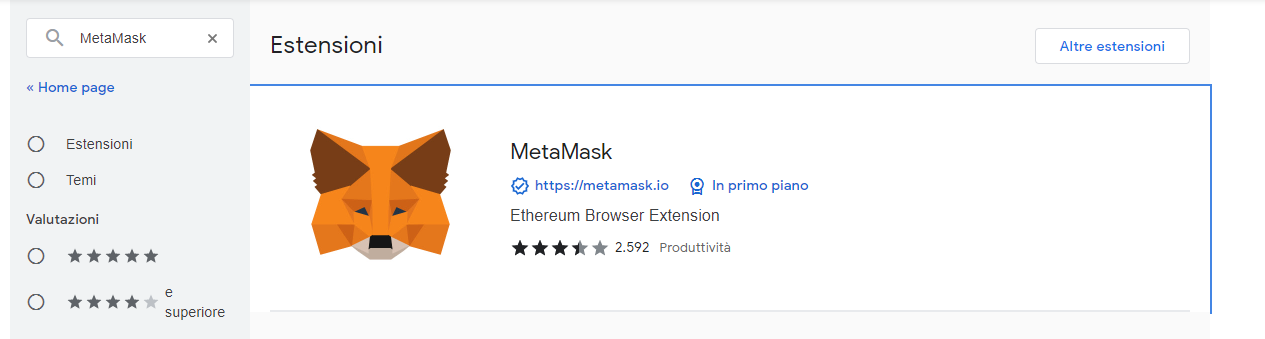
\includegraphics[scale = 0.4]{img/Estensione1.PNG}\\
    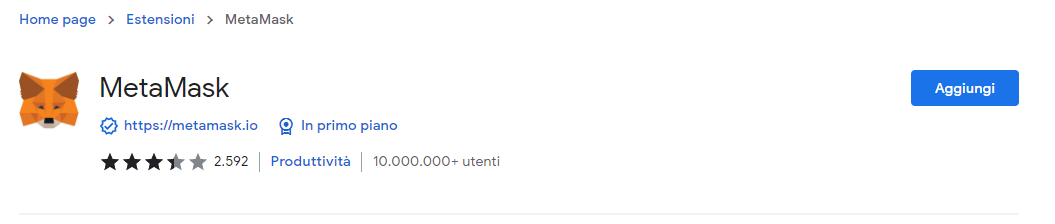
\includegraphics[scale = 0.4]{img/Estensione2.PNG}
    \item Una volta aggiunta l’estensione, cliccare sopra l’icona di MetaMask sulla barra estensioni per accedere alla schermata di benvenuto.\\
     \begin{center}
        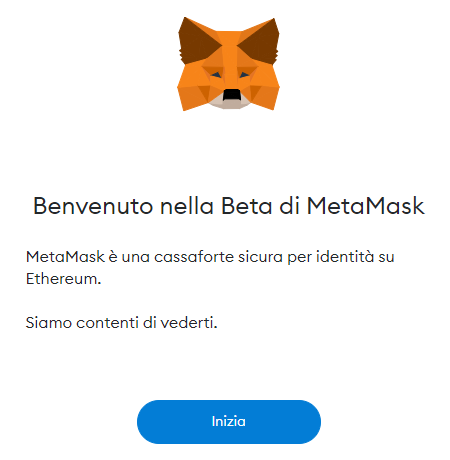
\includegraphics[scale = 0.4]{img/MetaMask1.PNG}
    \end{center}
    \item Cliccare su "Inizia" -> "Crea un portafoglio", accettare i termini d’uso e creare una password \\
         \begin{center}
    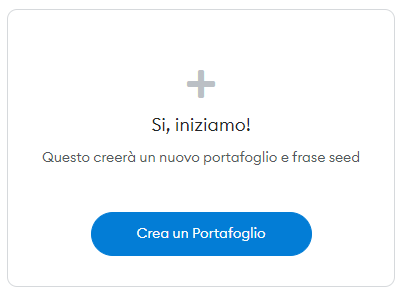
\includegraphics[scale = 0.4]{img/Wallet.PNG}
    \end{center}
    \item Andare avanti con la procedura e ricordarsi di scrivere la propria \textbf{SECRET RECOVERY PHRASE} su più mezzi di informazioni per recuperare il wallet in caso di necessità e dopo aver superato il test per la conferma della SECRET RECOVERY PHASE, la procedurà terminerà.
    
\end{enumerate}

\subsubsection{Creazione wallet MetaMask (mobile)}

Di seguito i passaggi necessari per creare un wallet su MetaMask tramite dispositivo mobile

\begin{enumerate}
    \item Andare nello Store del proprio dispositivo e digitare nella barra di ricerca "MetaMask". Successivamente fare tap sul bottone per avviare il download dell'App. \\
    \begin{center}
        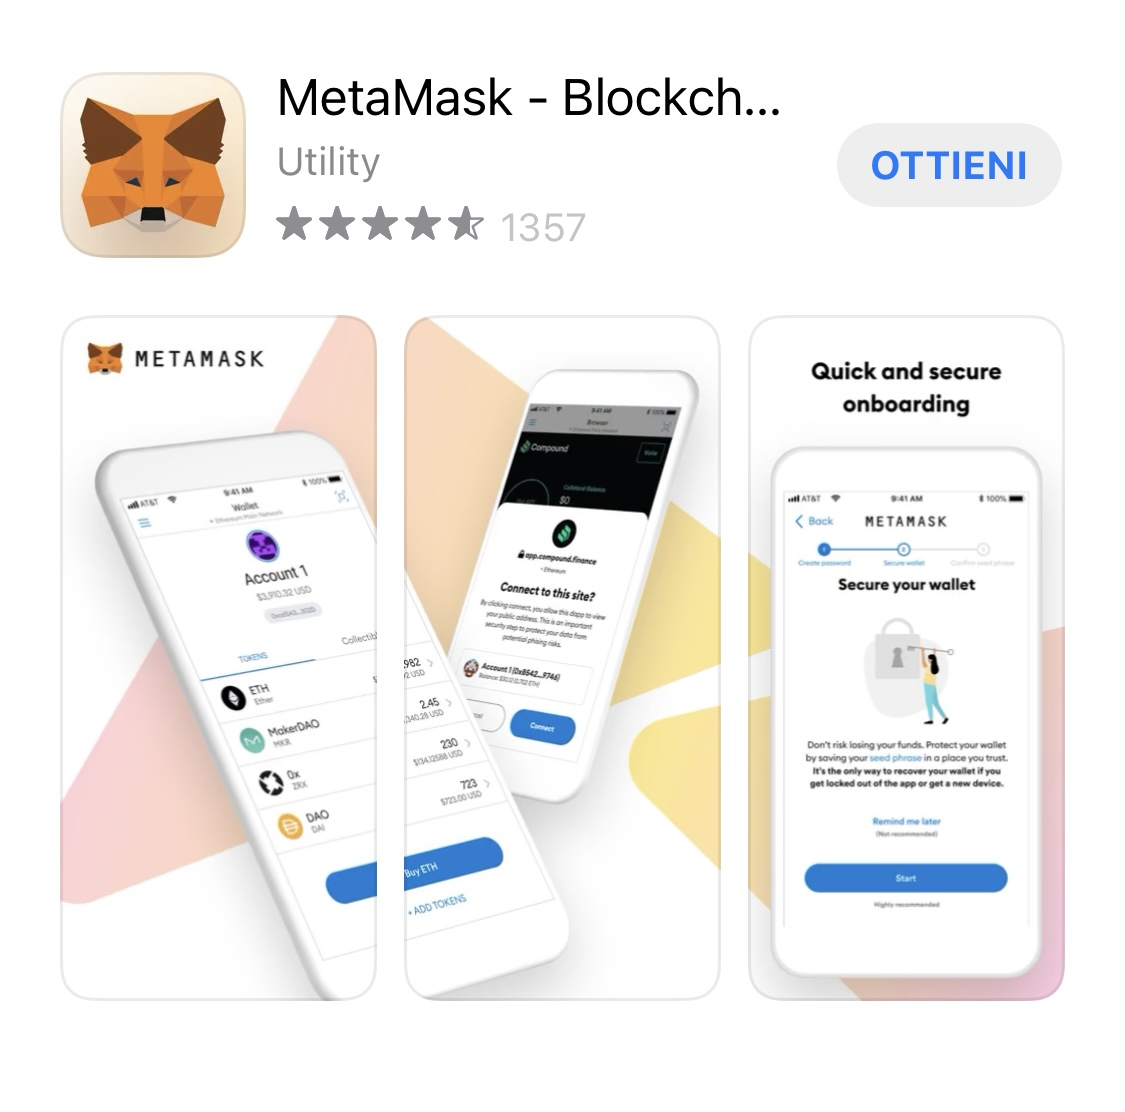
\includegraphics[scale = 0.2]{img/metamask_mobile_store1.jpg}\\
    \end{center}
    
    \item Dopo aver completato il download di MetaMask, aprire l'App dal menu del proprio dispositivo mobile. Nella schermata iniziale fare tap su "Get Started".
     \begin{center}
        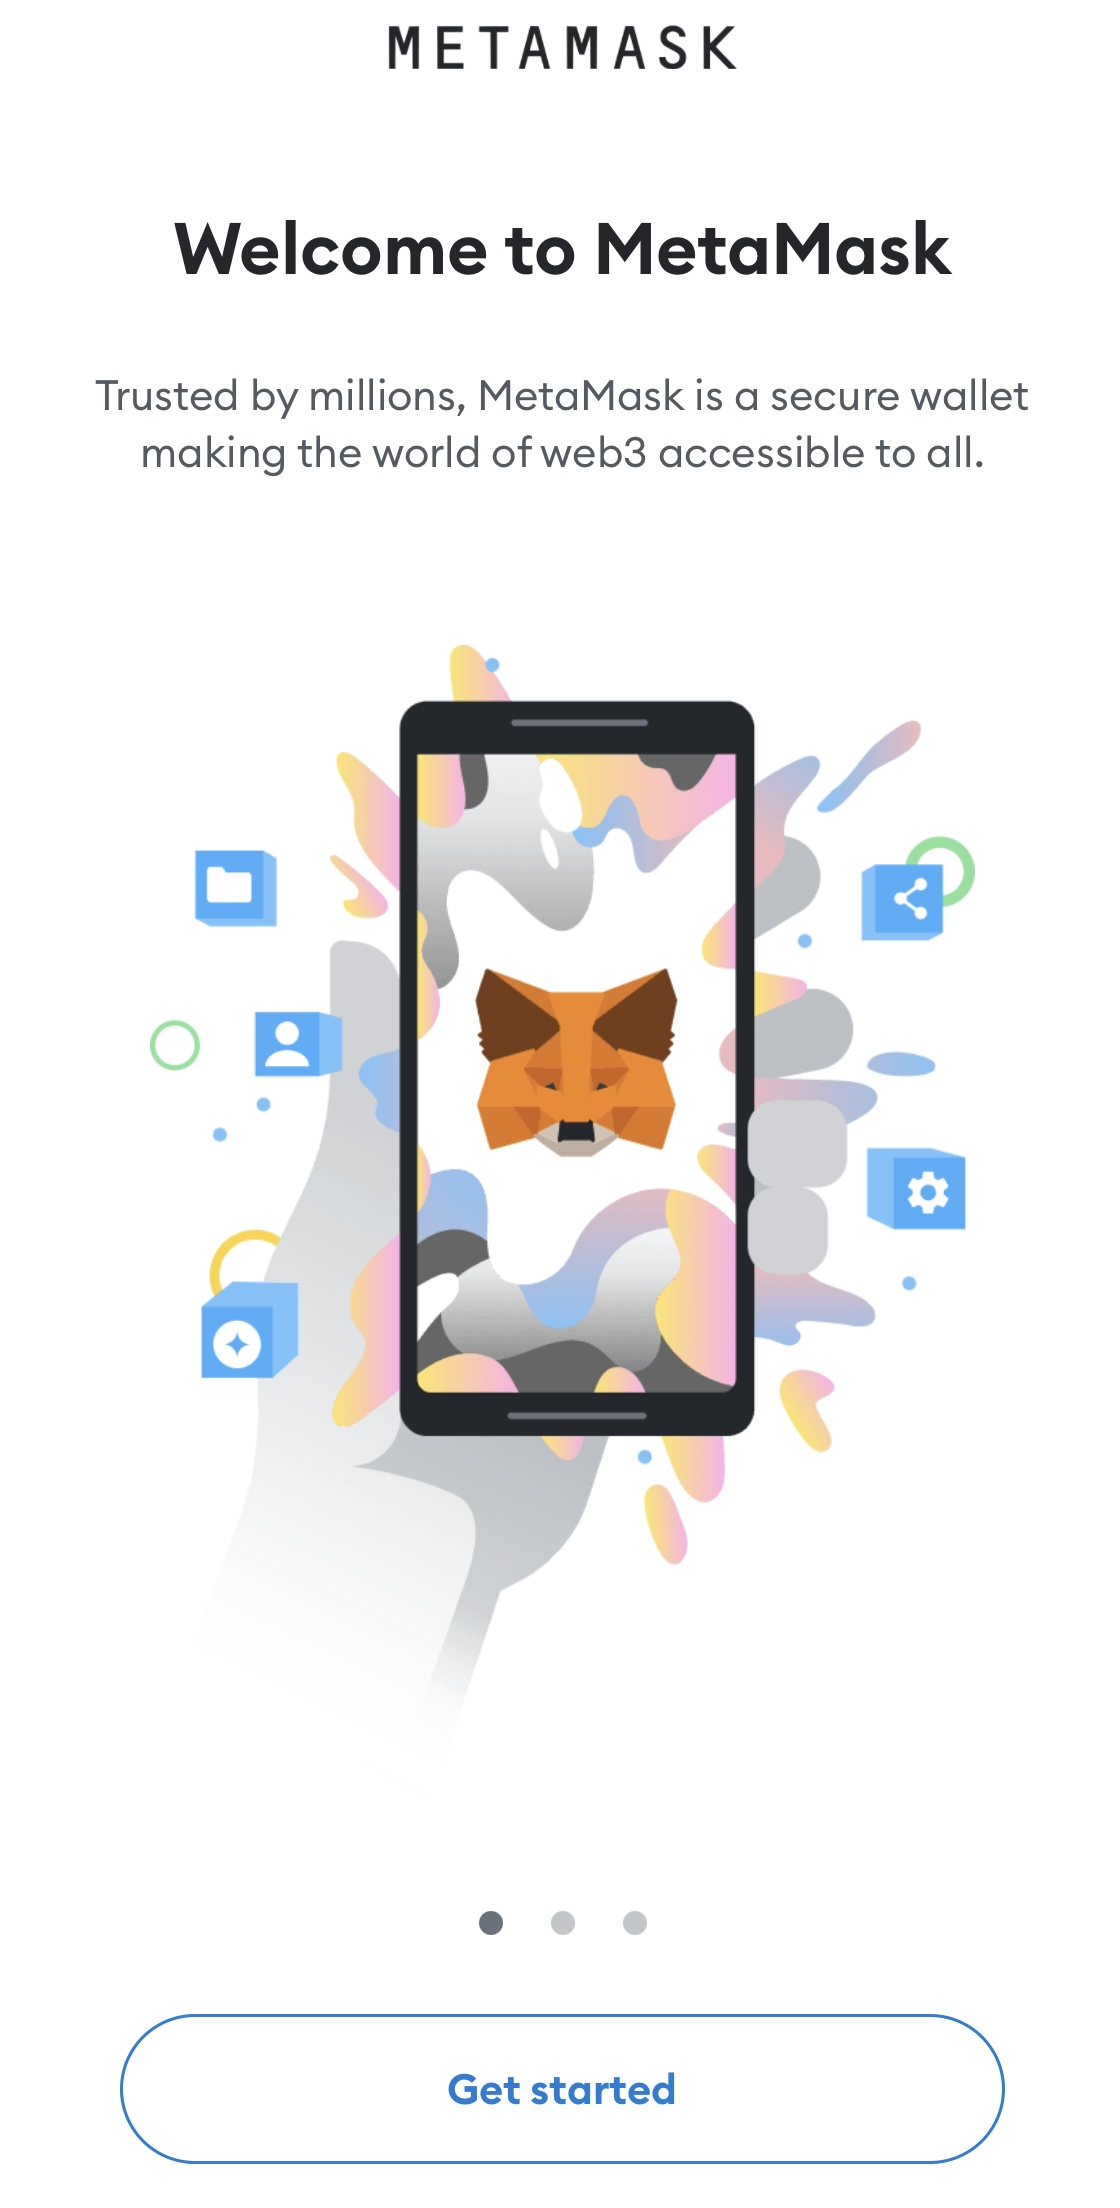
\includegraphics[scale = 0.1]{img/metamask_mobile_store2.jpg}
    \end{center}
    
    \item Selezionare "Create new wallet", dopo aver accettato i termini d'uso è possibile creare una password. \\
         \begin{center}
    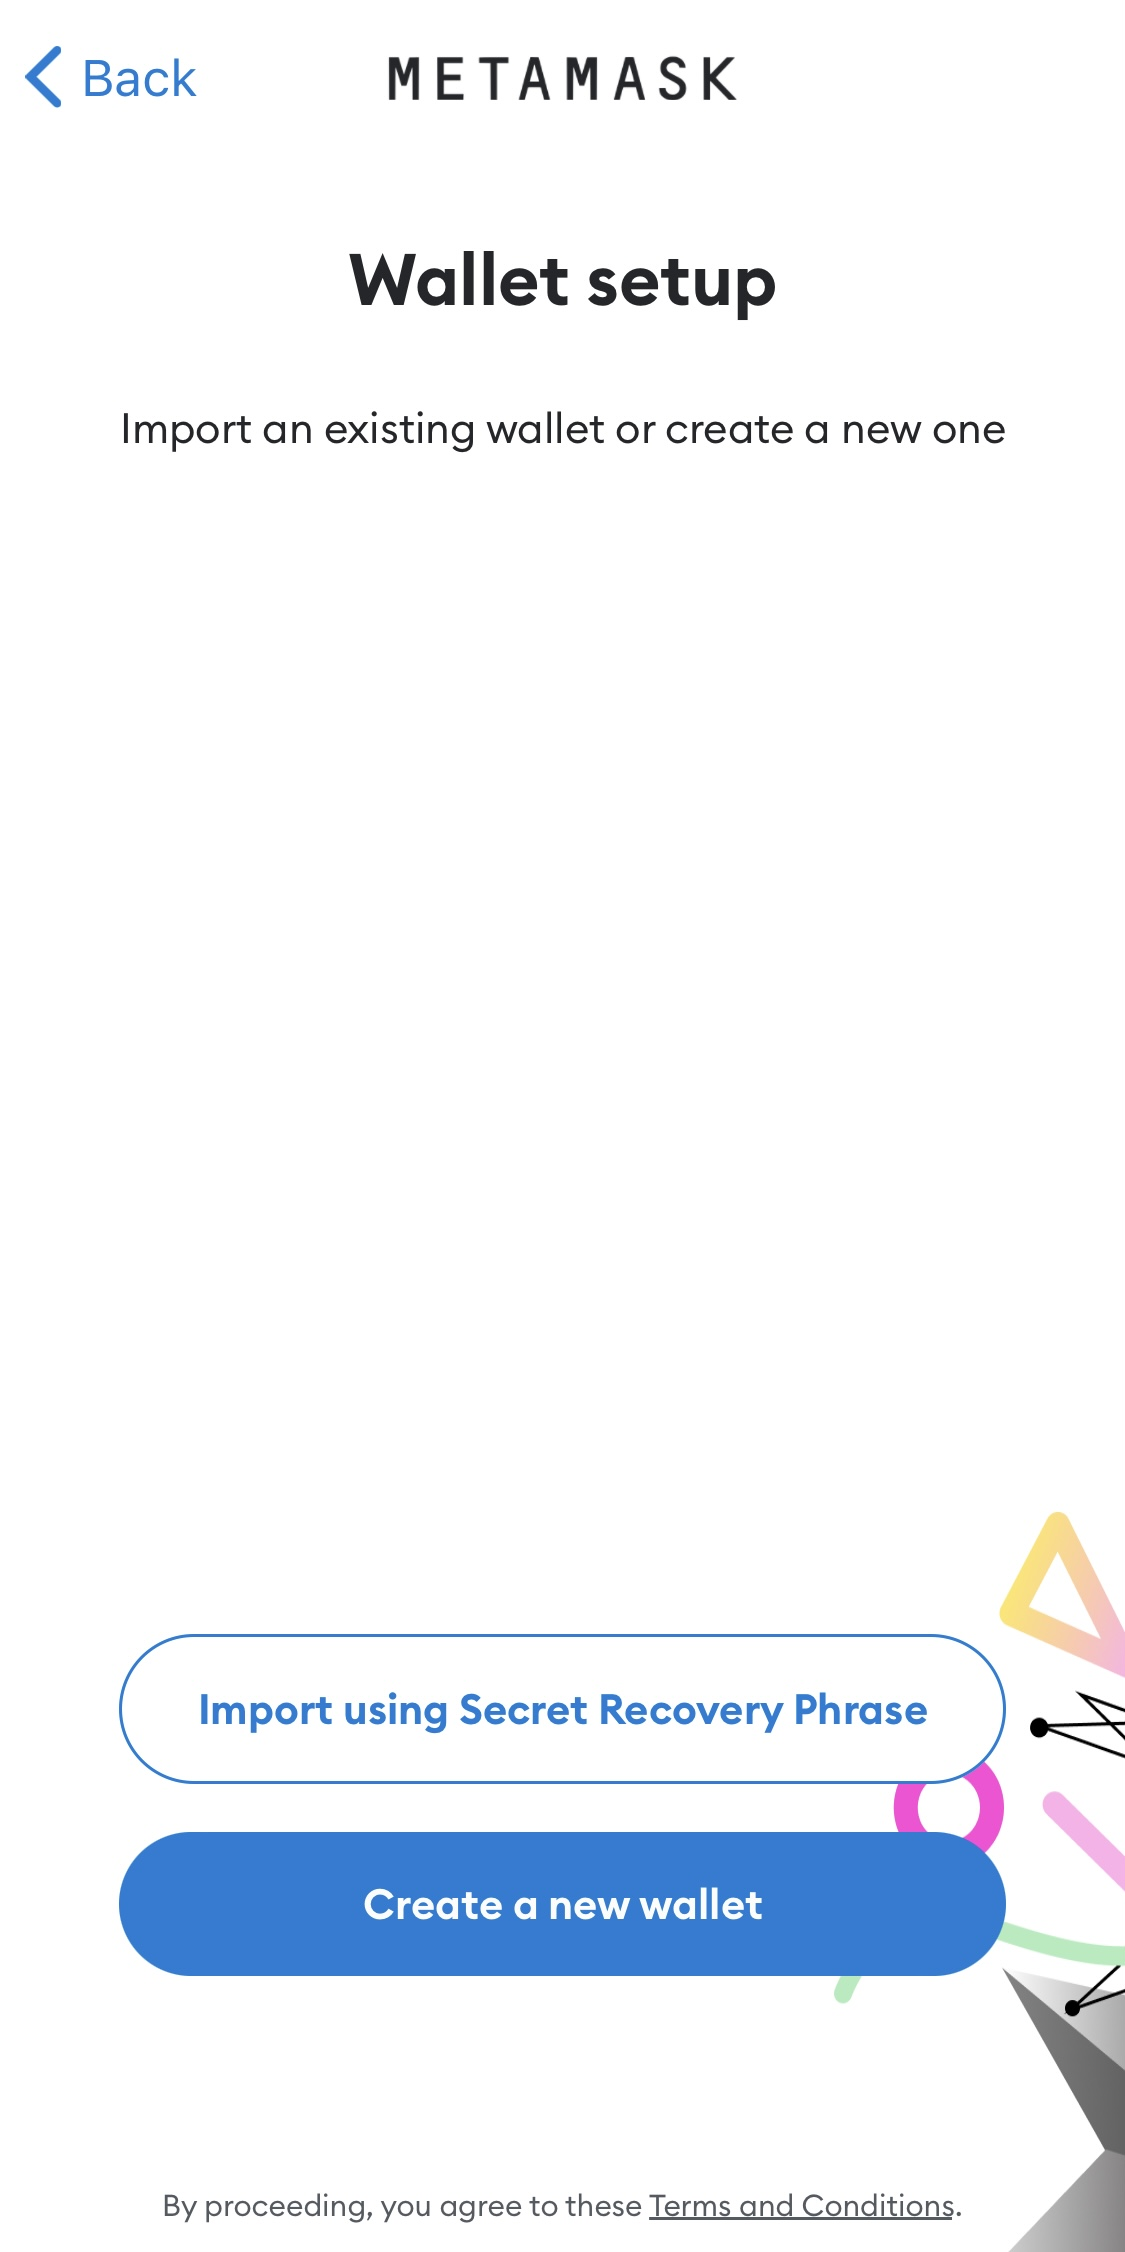
\includegraphics[scale = 0.1]{img/metamask_mobile_store3.jpg}
    \end{center}
    
    \item Seguire le istruzione per completare la procedura. È importante ricordarsi di annotare la \textbf{SECRET RECOVERY PHRASE} in modo tale da recuperare il wallet se necessario.
    
\end{enumerate}
\subsection{Web App}

\subsubsection{Collegamento Wallet}

\begin{enumerate}
    \item Una volta aperta la pagina principale di ShopChain sarà possibile connette il proprio wallet tramite MetaMask. \\


\begin{center}
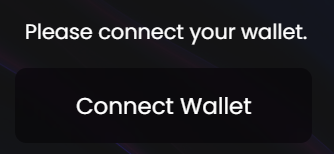
\includegraphics[scale = 0.5]{img/Connect.PNG}\\
\end{center}

Notifica di MetaMask:\\
\begin{center}
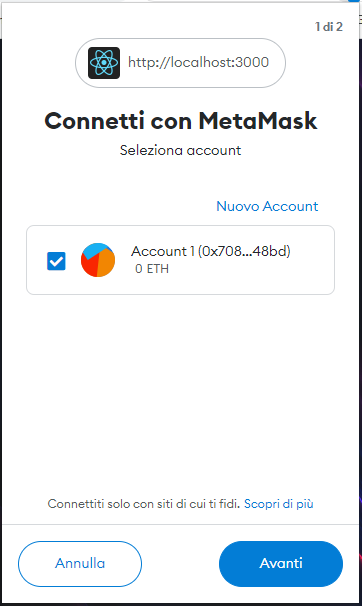
\includegraphics[scale = 0.4]{img/connessioneAvanti.PNG}\\
\end{center}

\item Nel caso in cui ci si trovasse nella rete sbagliata per la transazione, ShopChain lo rileverà in modo automatico e verrà chiesto di cambiarla. \\



\begin{center}
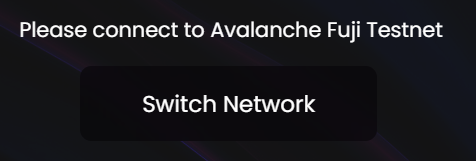
\includegraphics[scale = 0.5]{img/SwitchNetwork.PNG}\\
\end{center}

Notifica di MetaMask:\\
\begin{center}
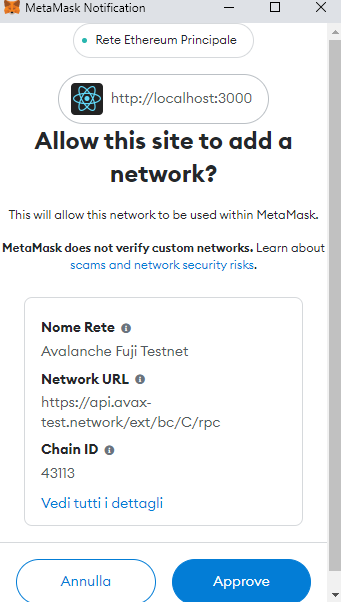
\includegraphics[scale = 0.5]{img/SwitchNetworkMetamask.PNG}
\end{center}

\item Quindi ci si ritroverà nella schermata Home:\\

\begin{center}
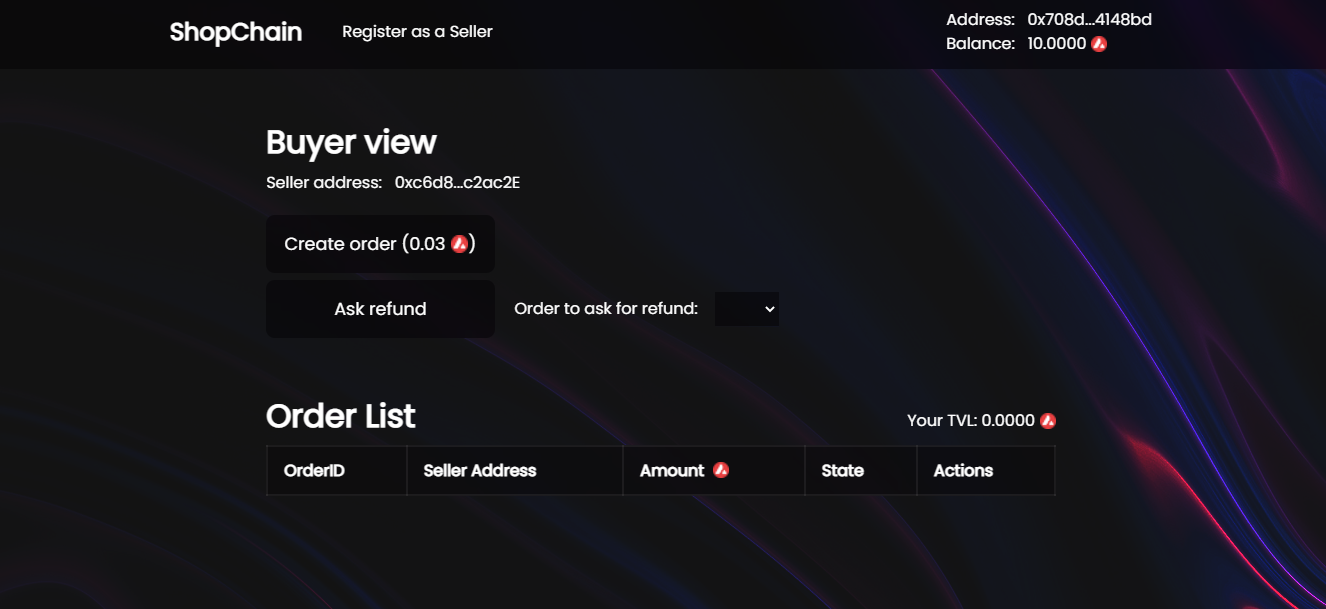
\includegraphics[scale = 0.35]{img/home.PNG}
\end{center}

\end{enumerate}
\subsubsection{Registrazione come Seller}

\begin{enumerate}
    \item Per registrarsi come seller è sufficiente cliccare l’opzione sulla barra menù "Register as Seller", dopodichè cliccare su Register.
    
    \begin{center}
        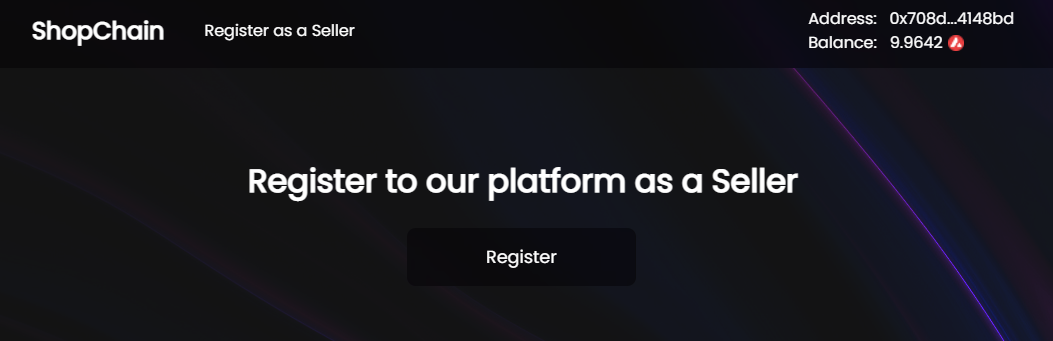
\includegraphics[scale = 0.4]{img/RegisterSeller.PNG}
    \end{center}
\end{enumerate}

\subsubsection{Creazione ordine}
\begin{enumerate}
    \item Per la creazione dell'ordine, dalla home, si clicchi sul pulsante "Create Order" dopodichè proseguire andando avanti su MetaMask.\\
    Notifica di MetaMask:\\
    \begin{center}
    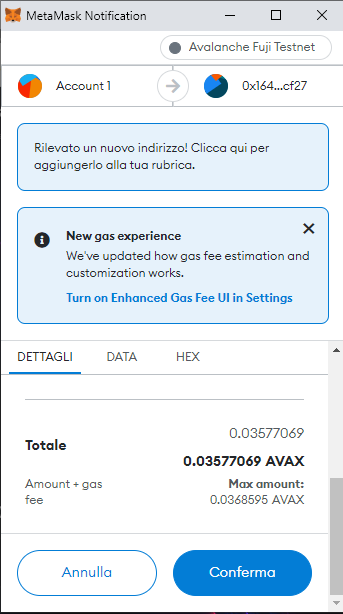
\includegraphics[scale = 0.35]{img/NotificaCrea Ordine.PNG}
    \end{center}
    
    \item Si visualizzerà su SnowTrace il resoconto della transazione.
    \begin{center}
    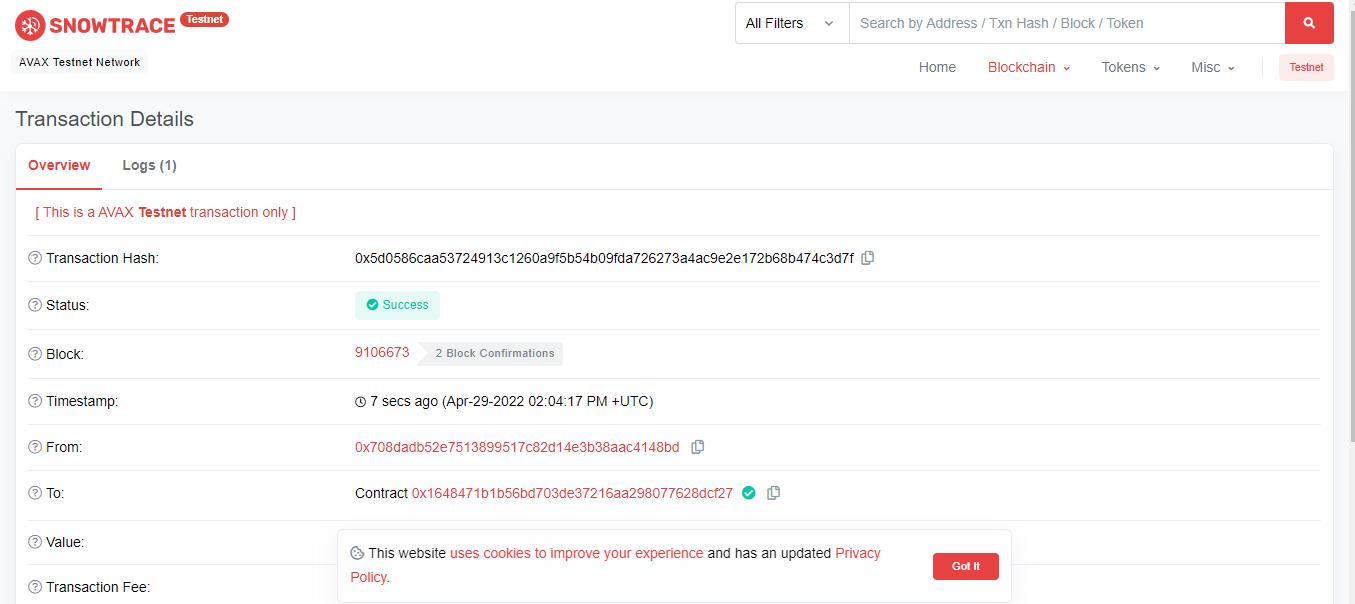
\includegraphics[scale = 0.35]{img/snowtrace.PNG}
    \end{center}
    
    \item Comparirà un nuovo record sulla tabella OrderList che descrive tutte le transazioni fatte dall'utente.
    
    \begin{center}
    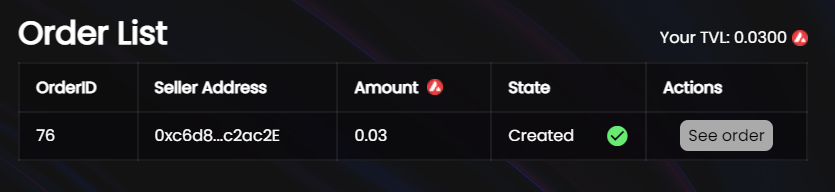
\includegraphics[scale = 0.35]{img/OrderList.PNG}\\
    \end{center}
    
\end{enumerate}

\subsubsection{Rimborso ordine}
\begin{enumerate}
    \item Per rimborsare l'ordine selezionare il corrispondente OrderID e schiacciare su "Ask Refund" e il TVL indica i soldi presenti nello SmartContract.
    
    Prima del refund\\
    \begin{center}
        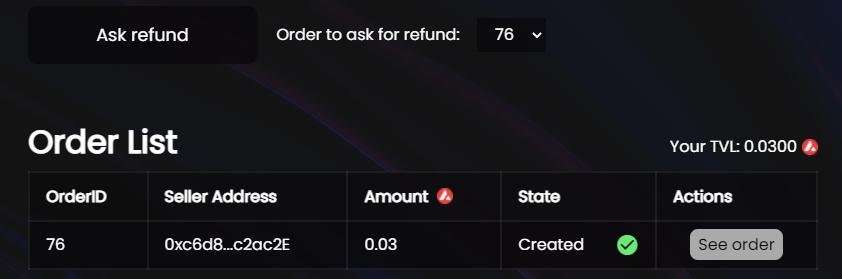
\includegraphics[scale = 0.35]{img/PrimaRefund.PNG}
    \end{center}  
    Dopo aver completato refund\\
    \begin{center}
        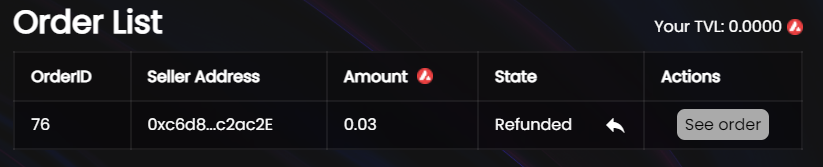
\includegraphics[scale = 0.35]{img/DopoRefund.PNG}
    \end{center}
\end{enumerate}

\pagebreak
\subsection{Mobile App}
\subsubsection{Collegamento Wallet}
\begin{enumerate}
    \item Una volta aperta l'app è necessario collegare il proprio wallet cliccando su "Connect Wallet.\\
    
    \begin{center}
        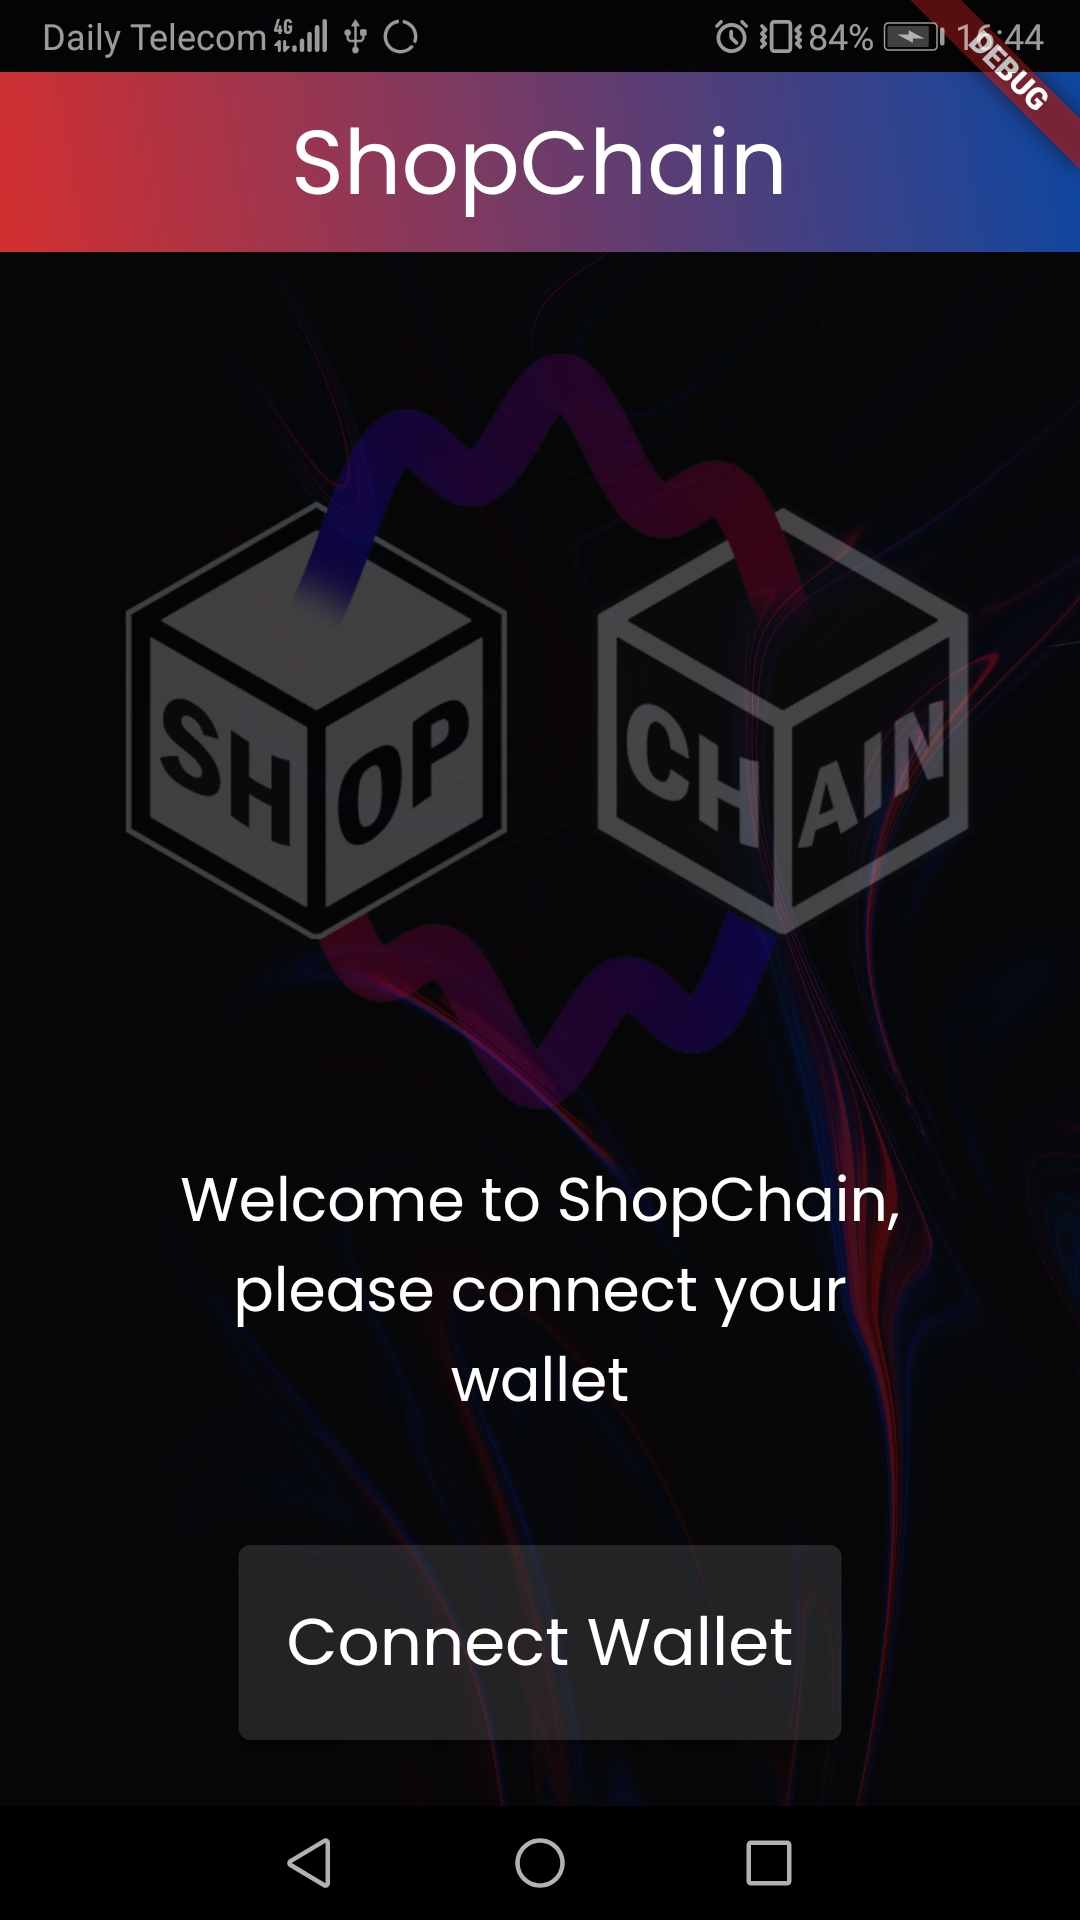
\includegraphics[scale = 0.1]{img/connectMobile.jpg}
    \end{center}
    
     \item Shopchain aprirà l'app di Metamask da dove si confermerà la connessione.\\
     \begin{center}
        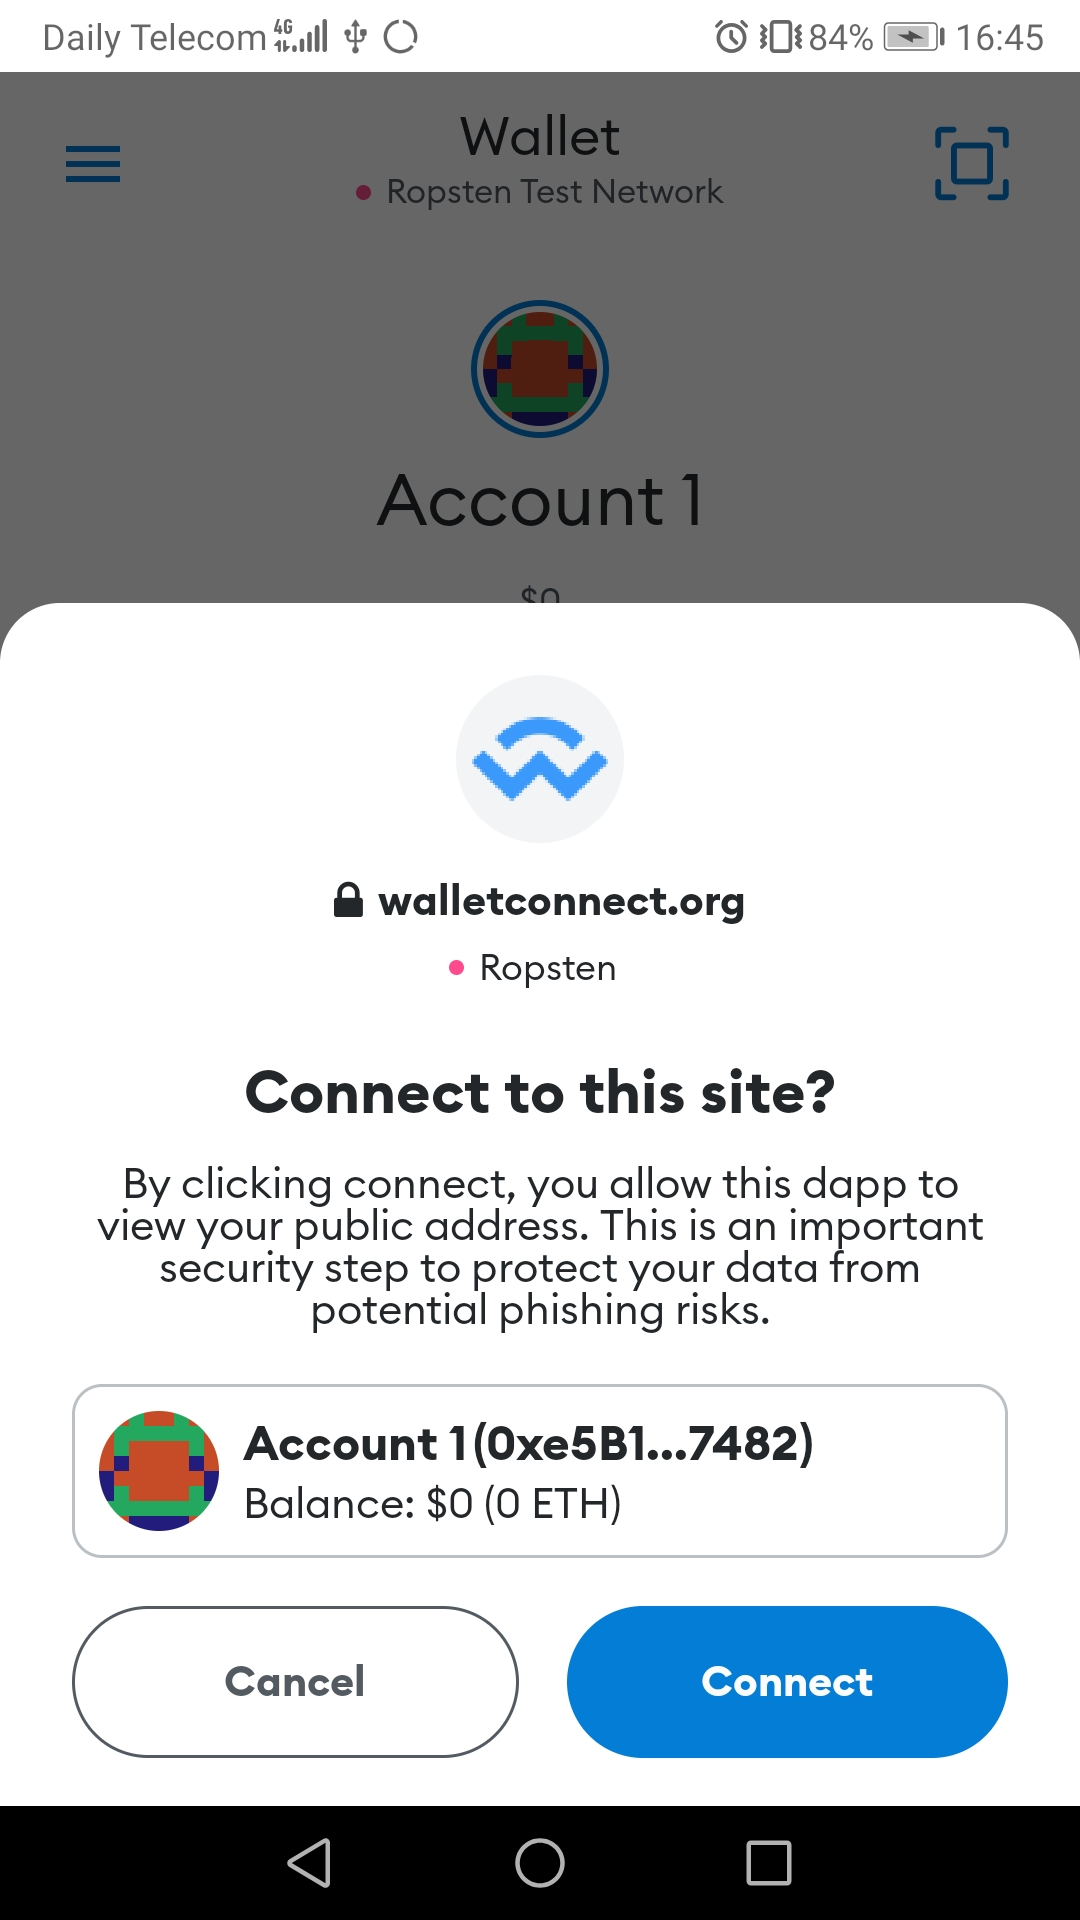
\includegraphics[scale = 0.1]{img/connectNotificaMobile.jpg}
    \end{center}
    
    \item Completata l'operazione ci si ritroverà nella Home:\\
     \begin{center}
        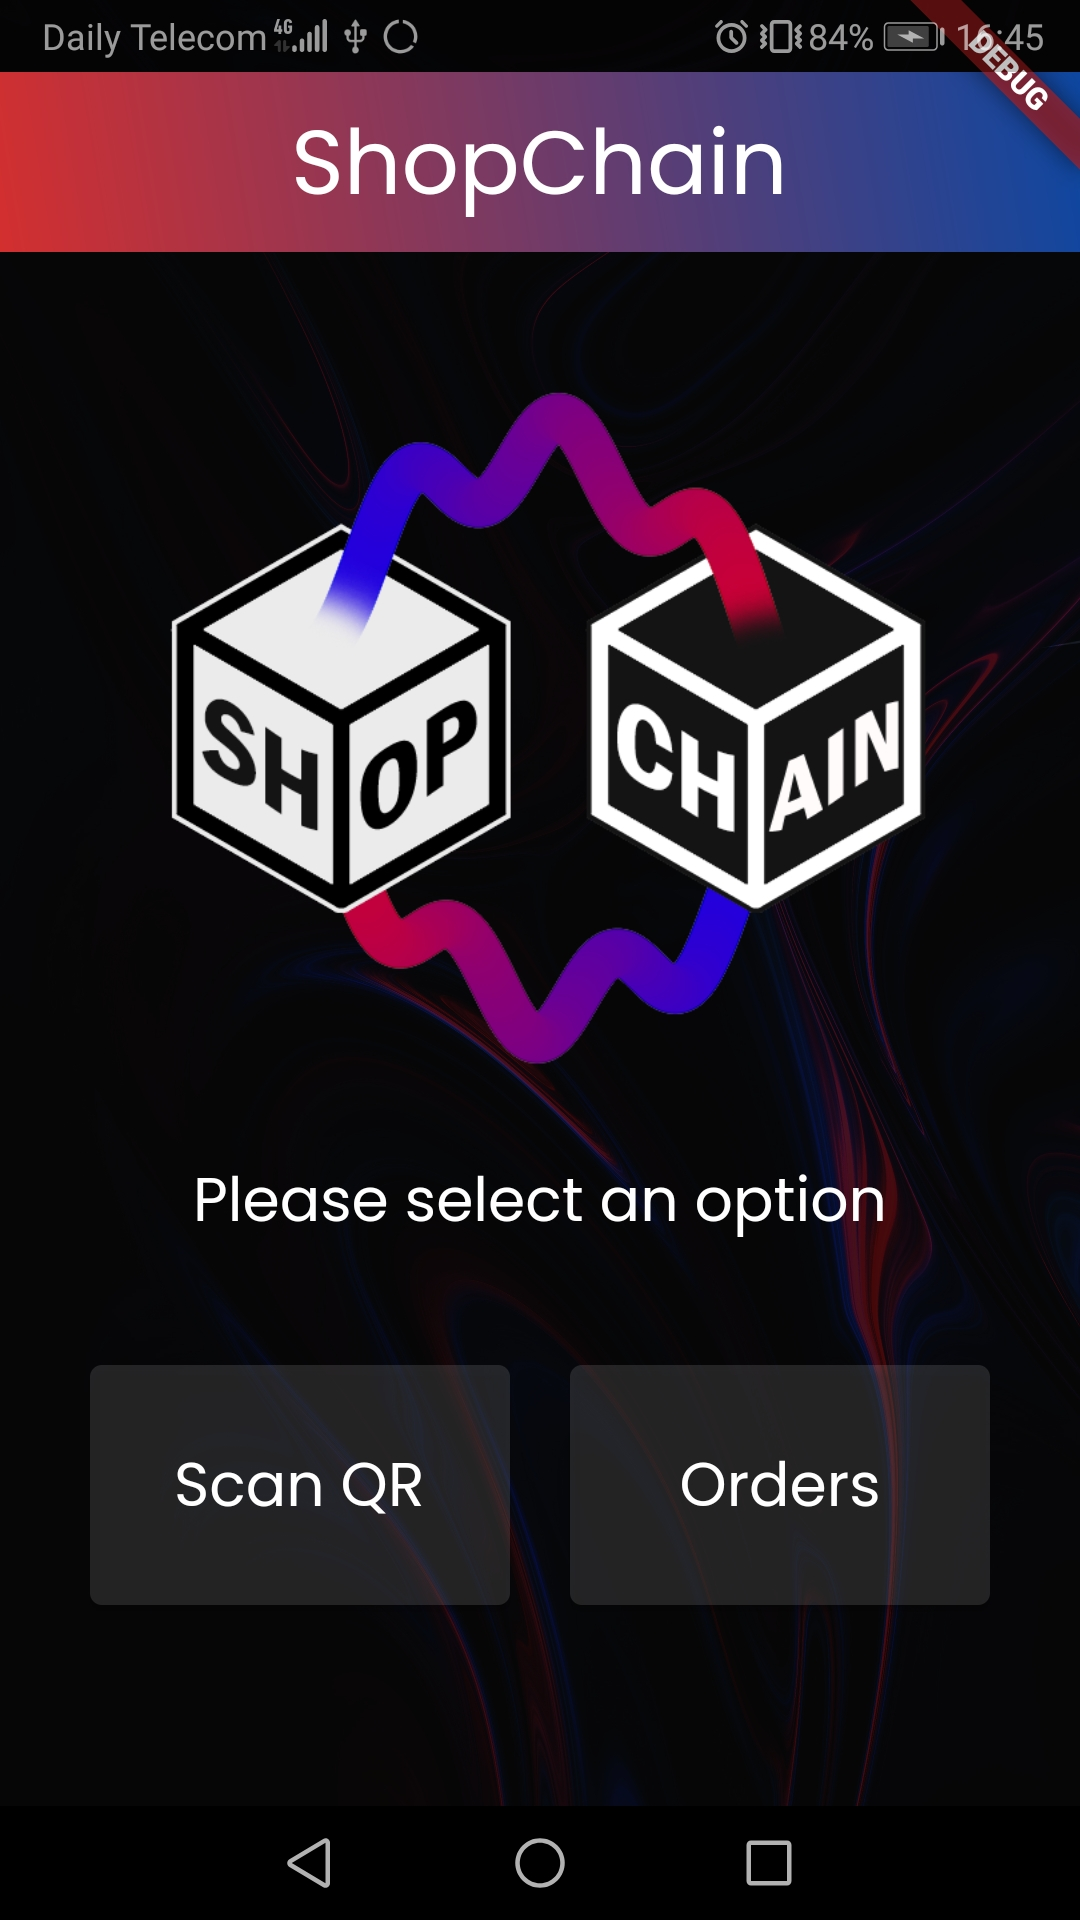
\includegraphics[scale = 0.1]{img/homeMobile.jpg}
    \end{center}
\end{enumerate}

\subsubsection{Scannerizzazione QRCode per ricezione ordine}
\begin{enumerate}
        \item Per scannerizzare un QR Code, partendo dalla Home, cliccare su "Scan QR"; si otterrà la seguente schermata: 
     \begin{center}
        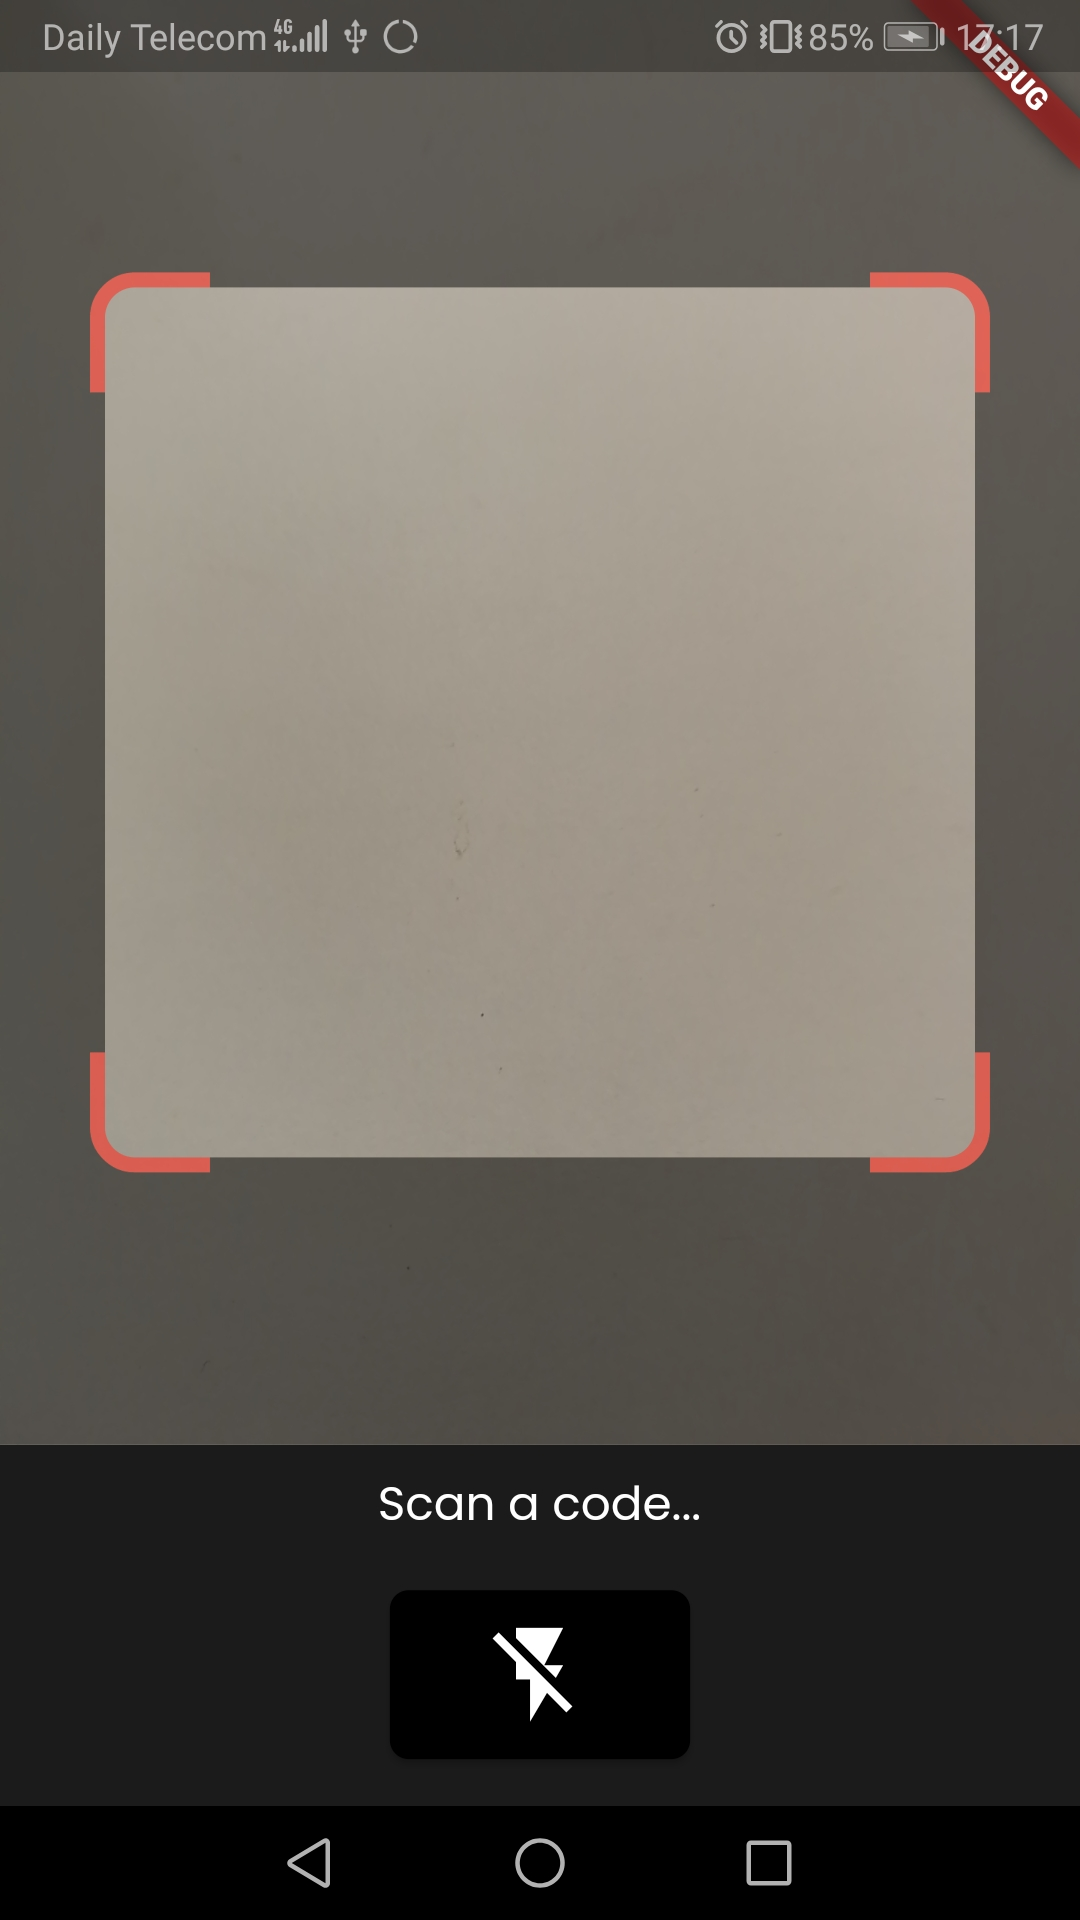
\includegraphics[scale = 0.1]{img/scanMobile.jpg}
    \end{center}
    \item Si può accendere/spegnere la torcia del telefono schiacciando sul pulsante con il simbolo dell'elettricità.
\end{enumerate}

\pagebreak

\subsubsection{Visualizzazione stato degli ordini}
\begin{enumerate}
    \item Per visualizzare lo stato degli ordini, partendo dalla Home, cliccare su "Orders"; si otterrà la seguente schermata: 
     \begin{center}
        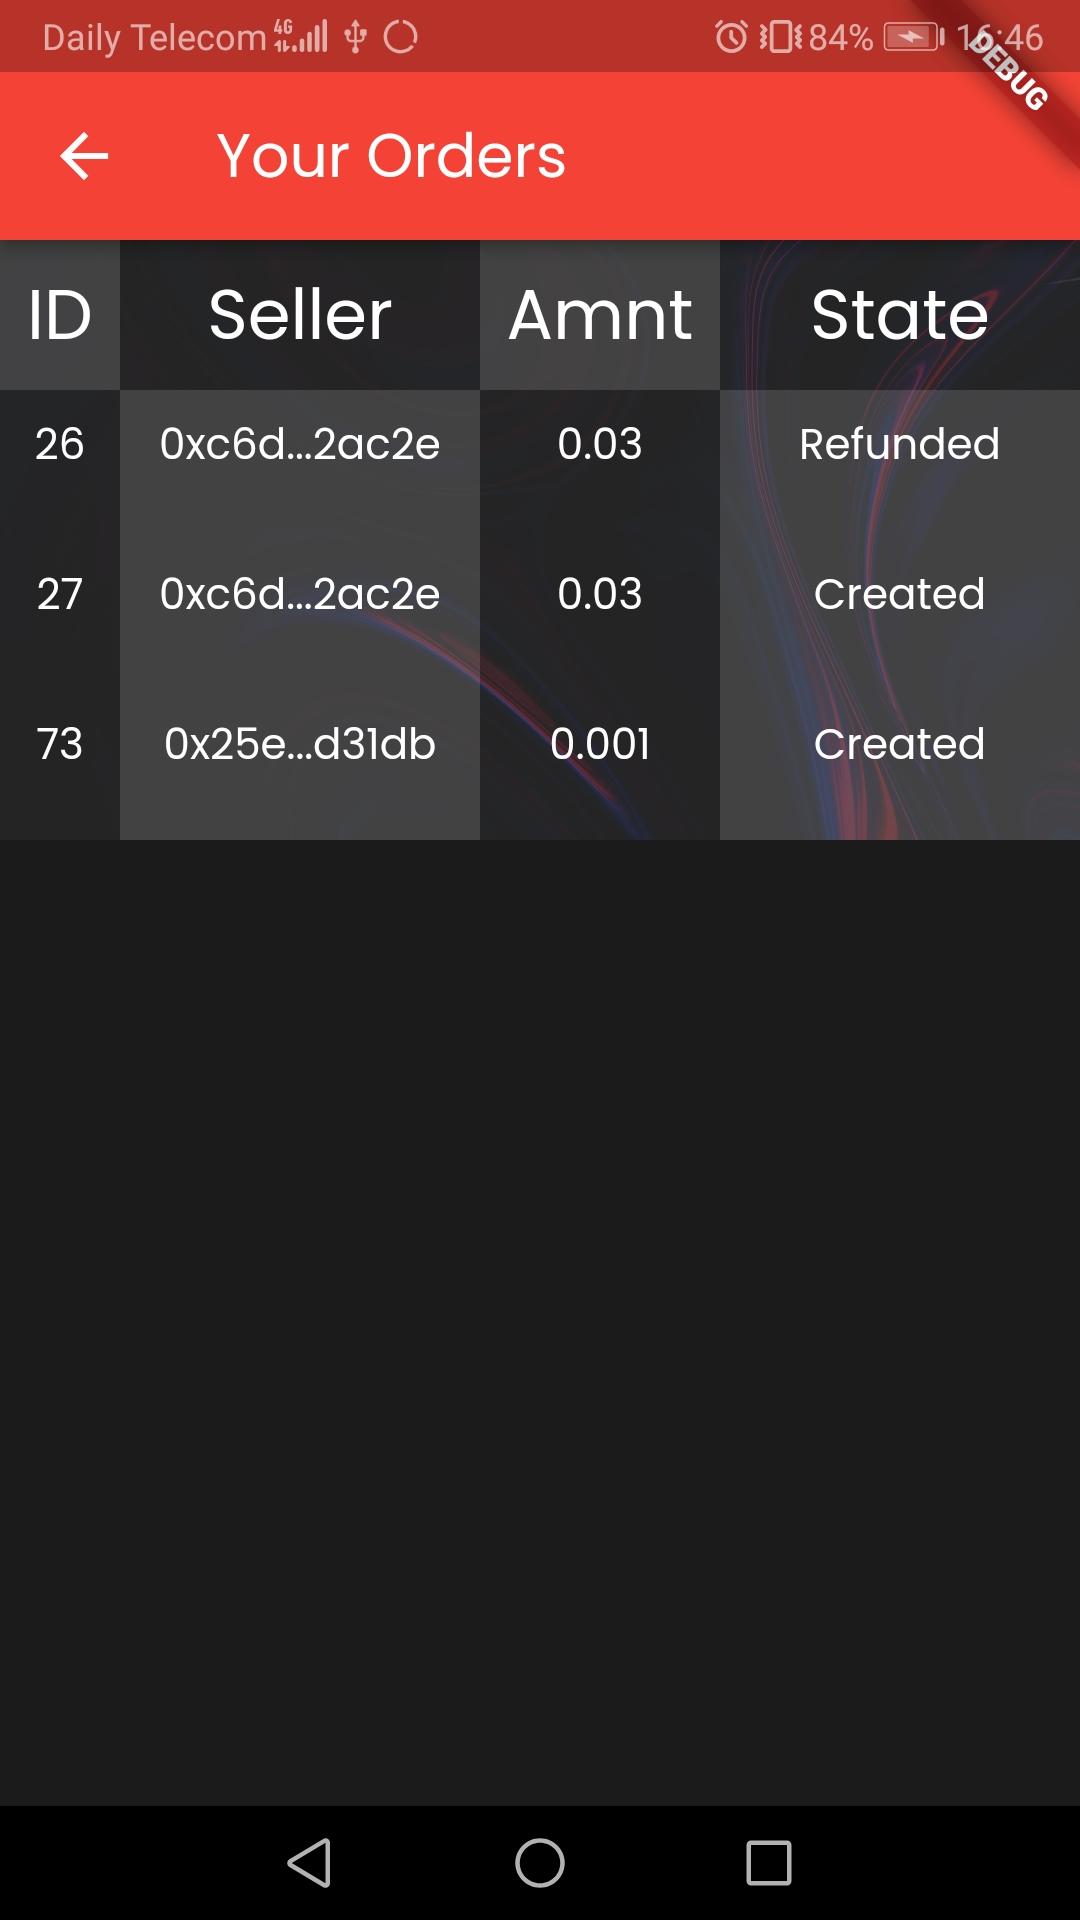
\includegraphics[scale = 0.1]{img/ordiniMobile.jpg}
    \end{center}
\end{enumerate}
